\documentclass[12]{article}

\usepackage{geometry}
\usepackage{amsmath, amsthm, amssymb}
\usepackage{graphicx}
\usepackage{tikz}
\usepackage{booktabs} % See the package documentation for guidelines on formal tables: https://ctan.org/pkg/booktabs
\usepackage{verbatim} % Used to typeset, for example, code snippets or pseudo-code for algorithms.
\usepackage{dsfont} % Extra fontset for helpful mathematics symbols, e.g. \mathds{1}
\usepackage{etoolbox} % Used to allow boolean variables for use in the title page
\usepackage{import}
\usepackage{lipsum}
\usepackage{subcaption}
\usepackage{float}
\usepackage{enumitem}
\usepackage{tabularx}
\usepackage{array}
\usepackage{pdfpages}
\usepackage{mathtools}
\usepackage{hyperref}
\newcolumntype{C}[1]{>{\centering\arraybackslash}m{#1}}
\newcommand{\R}{\mathbb{R}}
\newcommand{\Q}{\mathbb{Q}}
\newcommand{\C}{\mathbb{C}}
\newcommand{\N}{\mathbb{N}}
\newcommand{\Z}{\mathbb{Z}}
\newcommand{\T}{\mathbb{T}}
\newcommand{\cA}{\mathcal{A}}
\newcommand{\cB}{\mathcal{B}}
\newcommand{\cD}{\mathcal{D}}
\newcommand{\cP}{\mathcal{P}}
\newcommand{\cM}{\mathcal{M}}
\newcommand{\abs}[1]{\left\lvert #1 \right\rvert}
\newcommand{\norm}[1]{\left\lVert #1 \right\rVert}
\newcommand{\set}[2]{\left\{#1 \ : \ #2\right\}}
\newcommand{\conv}[1]{\underset{#1}\longrightarrow}
\newcommand{\Mod}[1]{\ (\mathrm{mod}\ #1)}
\newcommand{\Supp}[0]{\ \mathrm{Supp}\ }
\DeclarePairedDelimiter\ceil{\lceil}{\rceil}
\DeclarePairedDelimiter\floor{\lfloor}{\rfloor}
\DeclareMathOperator{\lcm}{lcm}
\newcommand{\Cross}{\mathbin{\tikz [x=1.4ex,y=1.4ex,line width=.2ex] \draw (0,0) -- (1,1) (0,1) -- (1,0);}}
% A custom restriction command, indicate that a function is being restricted to a subset of its domain.
\newcommand\restr[2]{{% we make the whole thing an ordinary symbol
		\left.\kern-\nulldelimiterspace % automatically resize the bar with \right
		#1 % the function
		\vphantom{\big|} % pretend it's a little taller at normal size
		\right|_{#2} % this is the delimiter
}}
% Custom math operators (analogous to \lim, \sup, etc).
\DeclareMathOperator{\id}{id}
\DeclareMathOperator{\subspan}{span}
\DeclareMathOperator{\sgn}{sgn}
% Custom List of ... commands. See the tocloft package documentation for more details.
% Any new lists of --- (for example, a List of Abbreviations, a List of Terms, etc) can be defined using the functionality in the package tocloft. This allows all lists in the preliminary pages to share the same formatting (as per UVic guidelines). 
% The following is a sample that you could use to include a list of abbreviations in the document.
% You could also create a glossary in a similar way.
%\newlistof[section]{abbrevs}{abr}{List of Abbreviations}
%\newcommand{\abbrevs}[2]{%   The command takes in two parameters: a phrase and its abbreviation.
	%	\refstepcounter{abbrevs}#1 (#2)% This line associates a number with the entry and typesets something there.
	%	\addcontentsline{abr}{abbrevs}{\numberline{}#2 - #1}}	% This line adds a line to the List of Abbreviations.
%--------------------------------------------------------------------------------------%
%								THEOREM ENVIRONMENTS
%--------------------------------------------------------------------------------------%
% Again, feel free to replace these with whatever is best for you! Look at the amsthm package documentation for more info.
% Tips for theorem numbering: While it's up to you, you might wish to try a system that makes it easiest to find results, and if two systems are equally easy to use, then use the simpler of the two. Generally you will have chapters or sections in your document, so numbering at least 1.1, 1.2, 2.1, 2.2, 2.3, ... might be good; if you also have subsections, maybe you could do 1.1.1, 1.1.2, 1.2.1, 1.2,2, etc, together with numbered subsections. You might also do unnumbered subsections and use only section numbering, if the subsections tend to be short.
% These environments are theorem-like; they have bold labels and italicized text. 
\newtheorem{thm}{Theorem}[section] % Numbering is impacted by [chapter]; could do [section] or [subsection] also.
\newtheorem{lem}{Lemma} % The [thm] argument says to number Lemma in sequence with Theorem.
\newtheorem{prop}[thm]{Proposition}
\newtheorem{cor}[thm]{Corollary}
\newtheorem{conj}[thm]{Conjecture}
\newtheorem{question}{Question}
% These environments are unnumbered and will not count toward the numbering.
%\newtheorem*{question}{Question}
\newtheorem*{answer}{Answer}
\newtheorem*{conjecture}{Conjecture}
\newtheorem*{claim}{Claim}
% These environments are definitions; they have a different style (bold label, standard font).
\theoremstyle{definition}
\newtheorem{defn}[thm]{Definition} % These definitions are also numbered in sequence with Theorem.
\newtheorem{eg}{Example}
\newtheorem{rem}[thm]{Remark}
\newtheorem{obs}{Observation}

\title{ \vspace{-3cm} Johnson Subgraph Problem Proposal }
\author{Tao Gaede}

\begin{document}
	\maketitle
	
	\begin{abstract}
		Summary
	\end{abstract}

	\section{Preliminaries}
	Let $J = J(n,k,i)$ be the graph with vertex set ${\Z_n \choose k}$ and for every $u,v \in V(J)$, $uv \in E(J)$ if and only if $|u \cap v| = k-i$ or equivalently $|u \Delta v| = 2i$.  We call $J(n,k,i)$ a \emph{Johnson graph}.
	
	We are interested in a particular class of induced subgraphs of $J(n,k,i)$, but we briefly introduce general Johnson induced subgraphs (JISs).  General induced subgraphs of $J(n,k,i)$ have apparently only been studied recently in the last 15 years or so. [Brief survey of literature on JISs]
	
	The class of JISs we aim to study are those whose vertices are characterized by a given pattern of consecutive differences.  By ``pattern of consecutive differences", we mean the following: Let $X \subseteq \Z_n$ and suppose $X = \{x_0,\ldots,x_{k-1}\}$ where $x_0 \leq \cdots \leq x_{k-1}$.  Then the pattern of consecutive differences for $X$, denoted $N_X$, is $N_X = (x_1-x_0,x_2-x_1,\ldots,x_{k-1} - x_{k-2}, x_0 - x_{k-1})$; additionally, we consider $N_X$ to be rotationally invariant, so all we care about is the cyclic ordering of the consecutive differences.  Note that $N_X$ is an \emph{integer necklace with $k$ beads of at most $n$ colours}.    Let $N$ be an integer necklace with $k$ beads of at most $n$ colours.  Then define $\mathcal{F}_N \subset {\Z_n \choose k}$ where for every $X \in \mathcal{F}_N$, $N_X = N$.  Observe that $\mathcal{F}_N$ is closed under taking translates, so for every $X,Y \in \mathcal{F}_N$, $Y = X + t$ for some $t \in \Z_n$ and $|\mathcal{F}_N| = n$.  The primary structure of interest is the subgraph of $J(n,k,i)$ induced by $\mathcal{F}_N$ for a given $n,k,i$, and $N$; we denote this subgraph by $JS(\mathcal{F}_N,i)$.
	
	[Examples of JISs for]
	
	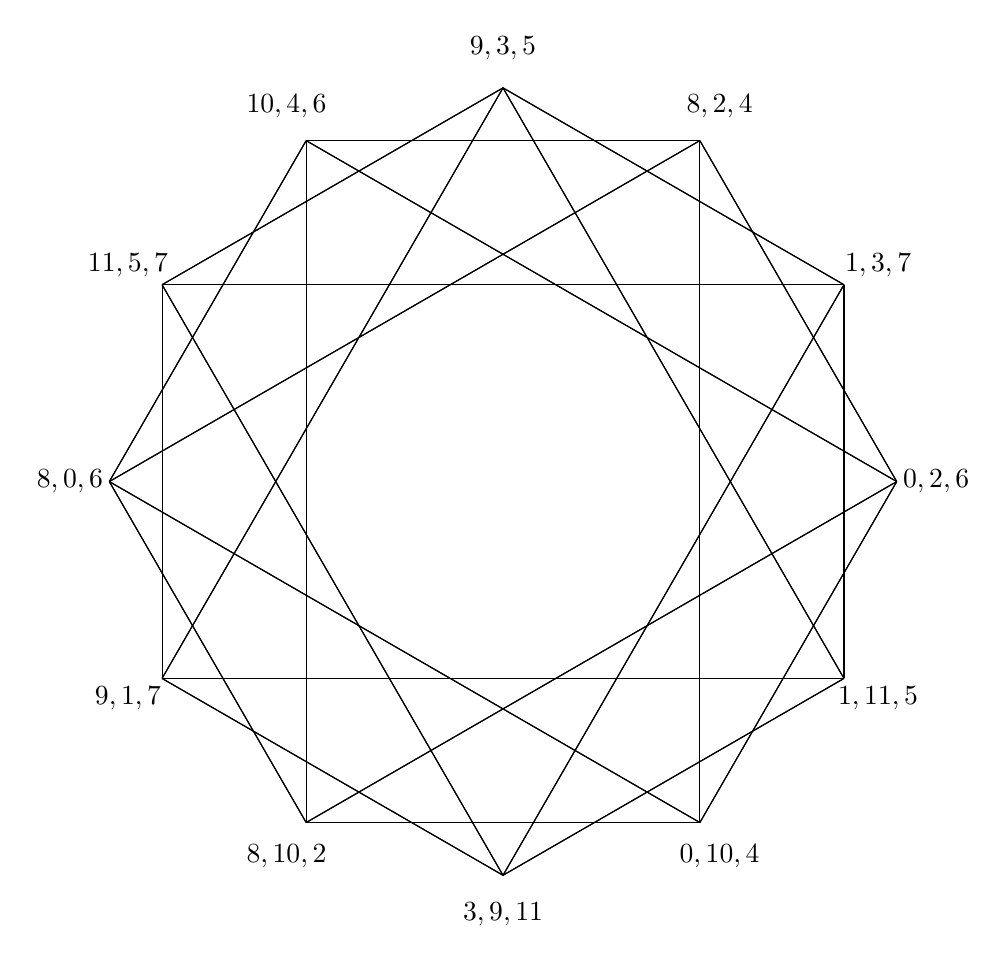
\begin{tikzpicture}
		\draw[black] ( 0  : 5)--( 60  : 5);
		\draw[black] ( 0  : 5)--( 120  : 5);
		\draw[black] ( 0  : 5)--( 240  : 5);
		\draw[black] ( 0  : 5)--( 300  : 5);
		\draw[black] ( 30  : 5)--( 90  : 5);
		\draw[black] ( 30  : 5)--( 150  : 5);
		\draw[black] ( 30  : 5)--( 270  : 5);
		\draw[black] ( 30  : 5)--( 330  : 5);
		\draw[black] ( 60  : 5)--( 0  : 5);
		\draw[black] ( 60  : 5)--( 120  : 5);
		\draw[black] ( 60  : 5)--( 180  : 5);
		\draw[black] ( 60  : 5)--( 300  : 5);
		\draw[black] ( 90  : 5)--( 30  : 5);
		\draw[black] ( 90  : 5)--( 150  : 5);
		\draw[black] ( 90  : 5)--( 210  : 5);
		\draw[black] ( 90  : 5)--( 330  : 5);
		\draw[black] ( 120  : 5)--( 0  : 5);
		\draw[black] ( 120  : 5)--( 60  : 5);
		\draw[black] ( 120  : 5)--( 180  : 5);
		\draw[black] ( 120  : 5)--( 240  : 5);
		\draw[black] ( 150  : 5)--( 30  : 5);
		\draw[black] ( 150  : 5)--( 90  : 5);
		\draw[black] ( 150  : 5)--( 210  : 5);
		\draw[black] ( 150  : 5)--( 270  : 5);
		\draw[black] ( 180  : 5)--( 60  : 5);
		\draw[black] ( 180  : 5)--( 120  : 5);
		\draw[black] ( 180  : 5)--( 240  : 5);
		\draw[black] ( 180  : 5)--( 300  : 5);
		\draw[black] ( 210  : 5)--( 90  : 5);
		\draw[black] ( 210  : 5)--( 150  : 5);
		\draw[black] ( 210  : 5)--( 270  : 5);
		\draw[black] ( 210  : 5)--( 330  : 5);
		\draw[black] ( 240  : 5)--( 0  : 5);
		\draw[black] ( 240  : 5)--( 120  : 5);
		\draw[black] ( 240  : 5)--( 180  : 5);
		\draw[black] ( 240  : 5)--( 300  : 5);
		\draw[black] ( 270  : 5)--( 30  : 5);
		\draw[black] ( 270  : 5)--( 150  : 5);
		\draw[black] ( 270  : 5)--( 210  : 5);
		\draw[black] ( 270  : 5)--( 330  : 5);
		\draw[black] ( 300  : 5)--( 0  : 5);
		\draw[black] ( 300  : 5)--( 60  : 5);
		\draw[black] ( 300  : 5)--( 180  : 5);
		\draw[black] ( 300  : 5)--( 240  : 5);
		\draw[black] ( 330  : 5)--( 30  : 5);
		\draw[black] ( 330  : 5)--( 90  : 5);
		\draw[black] ( 330  : 5)--( 210  : 5);
		\draw[black] ( 330  : 5)--( 270  : 5);
		\draw[fill=black] ( 0  : 5.5) node {$ {0, 2, 6} $};
		\draw[fill=black] ( 30  : 5.5) node {$ {1, 3, 7} $};
		\draw[fill=black] ( 60  : 5.5) node {$ {8, 2, 4} $};
		\draw[fill=black] ( 90  : 5.5) node {$ {9, 3, 5} $};
		\draw[fill=black] ( 120  : 5.5) node {$ {10, 4, 6} $};
		\draw[fill=black] ( 150  : 5.5) node {$ {11, 5, 7} $};
		\draw[fill=black] ( 180  : 5.5) node {$ {8, 0, 6} $};
		\draw[fill=black] ( 210  : 5.5) node {$ {9, 1, 7} $};
		\draw[fill=black] ( 240  : 5.5) node {$ {8, 10, 2} $};
		\draw[fill=black] ( 270  : 5.5) node {$ {3, 9, 11} $};
		\draw[fill=black] ( 300  : 5.5) node {$ {0, 10, 4} $};
		\draw[fill=black] ( 330  : 5.5) node {$ {1, 11, 5} $};
		%\draw[fill=black] (0 : 5) node {$\{1,2,3\}$};
		%\draw[fill=black] (90 : 5) circle (3pt);
	\end{tikzpicture}
	
	\begin{center}
	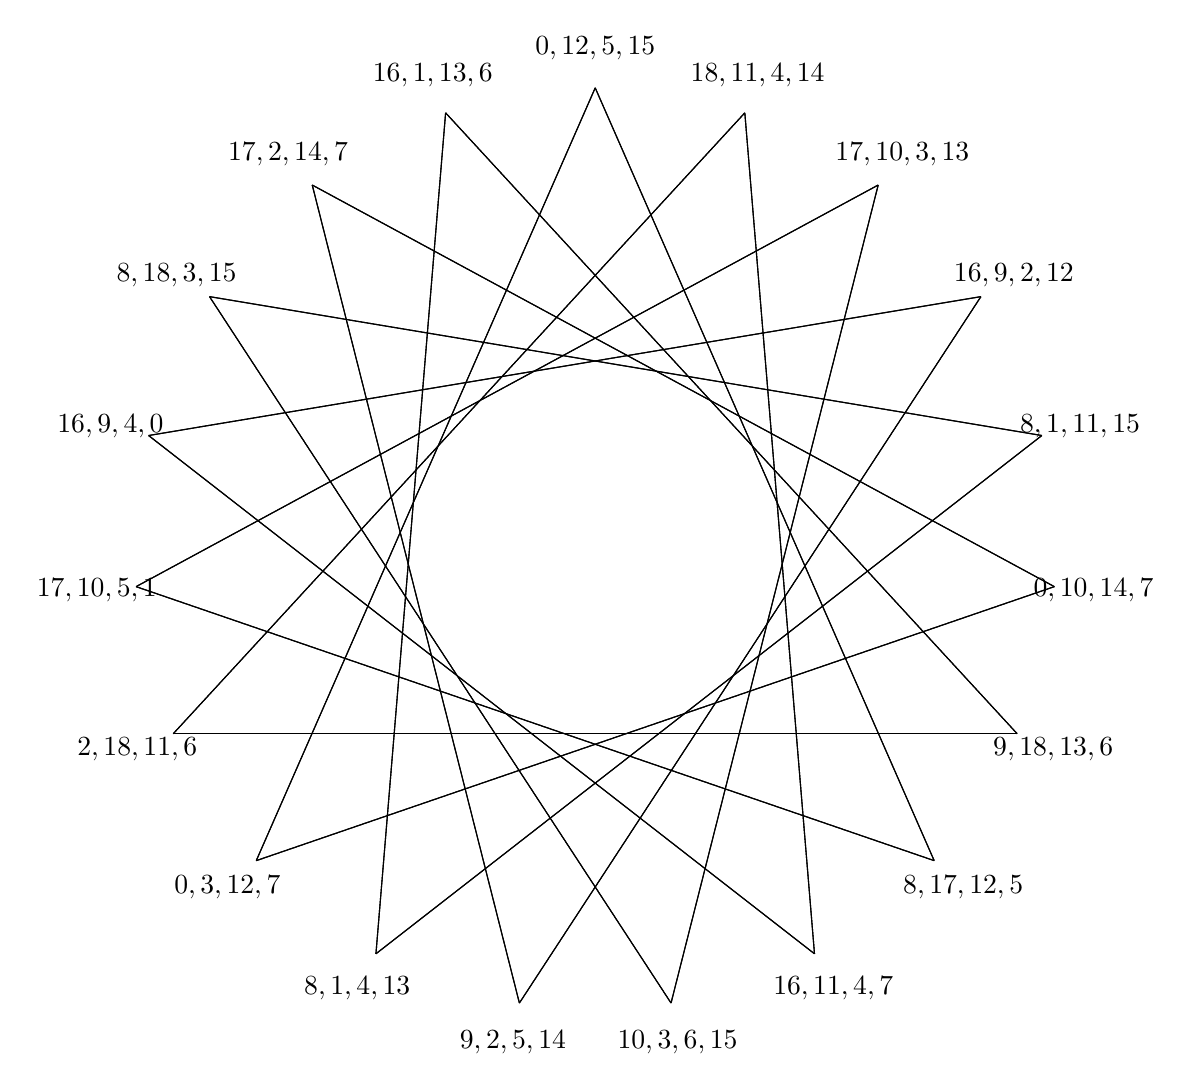
\begin{tikzpicture}
	\draw[black] ( 90  :  5.85129724240922 )--( 4230/19  :  5.85129724240922 );
	\draw[black] ( 90  :  5.85129724240922 )--( 6030/19  :  5.85129724240922 );
	\draw[black] ( 2070/19  :  5.85129724240922 )--( 4590/19  :  5.85129724240922 );
	\draw[black] ( 2070/19  :  5.85129724240922 )--( 6390/19  :  5.85129724240922 );
	\draw[black] ( 2430/19  :  5.85129724240922 )--( 4950/19  :  5.85129724240922 );
	\draw[black] ( 2430/19  :  5.85129724240922 )--( 6750/19  :  5.85129724240922 );
	\draw[black] ( 2790/19  :  5.85129724240922 )--( 5310/19  :  5.85129724240922 );
	\draw[black] ( 2790/19  :  5.85129724240922 )--( 7110/19  :  5.85129724240922 );
	\draw[black] ( 3150/19  :  5.85129724240922 )--( 5670/19  :  5.85129724240922 );
	\draw[black] ( 3150/19  :  5.85129724240922 )--( 7470/19  :  5.85129724240922 );
	\draw[black] ( 3510/19  :  5.85129724240922 )--( 6030/19  :  5.85129724240922 );
	\draw[black] ( 3510/19  :  5.85129724240922 )--( 7830/19  :  5.85129724240922 );
	\draw[black] ( 3870/19  :  5.85129724240922 )--( 6390/19  :  5.85129724240922 );
	\draw[black] ( 3870/19  :  5.85129724240922 )--( 8190/19  :  5.85129724240922 );
	\draw[black] ( 4230/19  :  5.85129724240922 )--( 90  :  5.85129724240922 );
	\draw[black] ( 4230/19  :  5.85129724240922 )--( 6750/19  :  5.85129724240922 );
	\draw[black] ( 4590/19  :  5.85129724240922 )--( 2070/19  :  5.85129724240922 );
	\draw[black] ( 4590/19  :  5.85129724240922 )--( 7110/19  :  5.85129724240922 );
	\draw[black] ( 4950/19  :  5.85129724240922 )--( 2430/19  :  5.85129724240922 );
	\draw[black] ( 4950/19  :  5.85129724240922 )--( 7470/19  :  5.85129724240922 );
	\draw[black] ( 5310/19  :  5.85129724240922 )--( 2790/19  :  5.85129724240922 );
	\draw[black] ( 5310/19  :  5.85129724240922 )--( 7830/19  :  5.85129724240922 );
	\draw[black] ( 5670/19  :  5.85129724240922 )--( 3150/19  :  5.85129724240922 );
	\draw[black] ( 5670/19  :  5.85129724240922 )--( 8190/19  :  5.85129724240922 );
	\draw[black] ( 6030/19  :  5.85129724240922 )--( 90  :  5.85129724240922 );
	\draw[black] ( 6030/19  :  5.85129724240922 )--( 3510/19  :  5.85129724240922 );
	\draw[black] ( 6390/19  :  5.85129724240922 )--( 2070/19  :  5.85129724240922 );
	\draw[black] ( 6390/19  :  5.85129724240922 )--( 3870/19  :  5.85129724240922 );
	\draw[black] ( 6750/19  :  5.85129724240922 )--( 2430/19  :  5.85129724240922 );
	\draw[black] ( 6750/19  :  5.85129724240922 )--( 4230/19  :  5.85129724240922 );
	\draw[black] ( 7110/19  :  5.85129724240922 )--( 2790/19  :  5.85129724240922 );
	\draw[black] ( 7110/19  :  5.85129724240922 )--( 4590/19  :  5.85129724240922 );
	\draw[black] ( 7470/19  :  5.85129724240922 )--( 3150/19  :  5.85129724240922 );
	\draw[black] ( 7470/19  :  5.85129724240922 )--( 4950/19  :  5.85129724240922 );
	\draw[black] ( 7830/19  :  5.85129724240922 )--( 3510/19  :  5.85129724240922 );
	\draw[black] ( 7830/19  :  5.85129724240922 )--( 5310/19  :  5.85129724240922 );
	\draw[black] ( 8190/19  :  5.85129724240922 )--( 3870/19  :  5.85129724240922 );
	\draw[black] ( 8190/19  :  5.85129724240922 )--( 5670/19  :  5.85129724240922 );
	\draw[fill=black] ( 90  :  6.35129724240922 ) node {$ {0, 12, 5, 15} $};
	\draw[fill=black] ( 2070/19  :  6.35129724240922 ) node {$ {16, 1, 13, 6} $};
	\draw[fill=black] ( 2430/19  :  6.35129724240922 ) node {$ {17, 2, 14, 7} $};
	\draw[fill=black] ( 2790/19  :  6.35129724240922 ) node {$ {8, 18, 3, 15} $};
	\draw[fill=black] ( 3150/19  :  6.35129724240922 ) node {$ {16, 9, 4, 0} $};
	\draw[fill=black] ( 3510/19  :  6.35129724240922 ) node {$ {17, 10, 5, 1} $};
	\draw[fill=black] ( 3870/19  :  6.35129724240922 ) node {$ {2, 18, 11, 6} $};
	\draw[fill=black] ( 4230/19  :  6.35129724240922 ) node {$ {0, 3, 12, 7} $};
	\draw[fill=black] ( 4590/19  :  6.35129724240922 ) node {$ {8, 1, 4, 13} $};
	\draw[fill=black] ( 4950/19  :  6.35129724240922 ) node {$ {9, 2, 5, 14} $};
	\draw[fill=black] ( 5310/19  :  6.35129724240922 ) node {$ {10, 3, 6, 15} $};
	\draw[fill=black] ( 5670/19  :  6.35129724240922 ) node {$ {16, 11, 4, 7} $};
	\draw[fill=black] ( 6030/19  :  6.35129724240922 ) node {$ {8, 17, 12, 5} $};
	\draw[fill=black] ( 6390/19  :  6.35129724240922 ) node {$ {9, 18, 13, 6} $};
	\draw[fill=black] ( 6750/19  :  6.35129724240922 ) node {$ {0, 10, 14, 7} $};
	\draw[fill=black] ( 7110/19  :  6.35129724240922 ) node {$ {8, 1, 11, 15} $};
	\draw[fill=black] ( 7470/19  :  6.35129724240922 ) node {$ {16, 9, 2, 12} $};
	\draw[fill=black] ( 7830/19  :  6.35129724240922 ) node {$ {17, 10, 3, 13} $};
	\draw[fill=black] ( 8190/19  :  6.35129724240922 ) node {$ {18, 11, 4, 14} $};
	\end{tikzpicture}
\end{center}

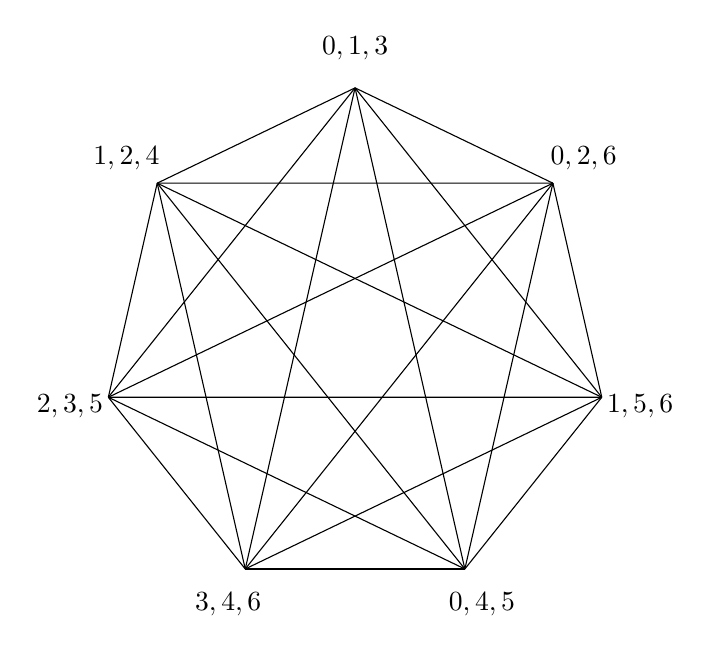
\begin{tikzpicture}
\draw[black] ( 90  :  3.21409584971604 )--( 990/7  :  3.21409584971604 );
\draw[black] ( 90  :  3.21409584971604 )--( 1350/7  :  3.21409584971604 );
\draw[black] ( 90  :  3.21409584971604 )--( 1710/7  :  3.21409584971604 );
\draw[black] ( 90  :  3.21409584971604 )--( 2070/7  :  3.21409584971604 );
\draw[black] ( 90  :  3.21409584971604 )--( 2430/7  :  3.21409584971604 );
\draw[black] ( 90  :  3.21409584971604 )--( 2790/7  :  3.21409584971604 );
\draw[black] ( 990/7  :  3.21409584971604 )--( 1350/7  :  3.21409584971604 );
\draw[black] ( 990/7  :  3.21409584971604 )--( 1710/7  :  3.21409584971604 );
\draw[black] ( 990/7  :  3.21409584971604 )--( 2070/7  :  3.21409584971604 );
\draw[black] ( 990/7  :  3.21409584971604 )--( 2430/7  :  3.21409584971604 );
\draw[black] ( 990/7  :  3.21409584971604 )--( 2790/7  :  3.21409584971604 );
\draw[black] ( 1350/7  :  3.21409584971604 )--( 1710/7  :  3.21409584971604 );
\draw[black] ( 1350/7  :  3.21409584971604 )--( 2070/7  :  3.21409584971604 );
\draw[black] ( 1350/7  :  3.21409584971604 )--( 2430/7  :  3.21409584971604 );
\draw[black] ( 1350/7  :  3.21409584971604 )--( 2790/7  :  3.21409584971604 );
\draw[black] ( 1710/7  :  3.21409584971604 )--( 2070/7  :  3.21409584971604 );
\draw[black] ( 1710/7  :  3.21409584971604 )--( 2430/7  :  3.21409584971604 );
\draw[black] ( 1710/7  :  3.21409584971604 )--( 2790/7  :  3.21409584971604 );
\draw[black] ( 2070/7  :  3.21409584971604 )--( 2430/7  :  3.21409584971604 );
\draw[black] ( 2070/7  :  3.21409584971604 )--( 2790/7  :  3.21409584971604 );
\draw[black] ( 2430/7  :  3.21409584971604 )--( 2790/7  :  3.21409584971604 );
\draw[fill=black] ( 90  :  3.71409584971604 ) node {$ {0, 1, 3} $};
\draw[fill=black] ( 990/7  :  3.71409584971604 ) node {$ {1, 2, 4} $};
\draw[fill=black] ( 1350/7  :  3.71409584971604 ) node {$ {2, 3, 5} $};
\draw[fill=black] ( 1710/7  :  3.71409584971604 ) node {$ {3, 4, 6} $};
\draw[fill=black] ( 2070/7  :  3.71409584971604 ) node {$ {0, 4, 5} $};
\draw[fill=black] ( 2430/7  :  3.71409584971604 ) node {$ {1, 5, 6} $};
\draw[fill=black] ( 2790/7  :  3.71409584971604 ) node {$ {0, 2, 6} $};
\end{tikzpicture}

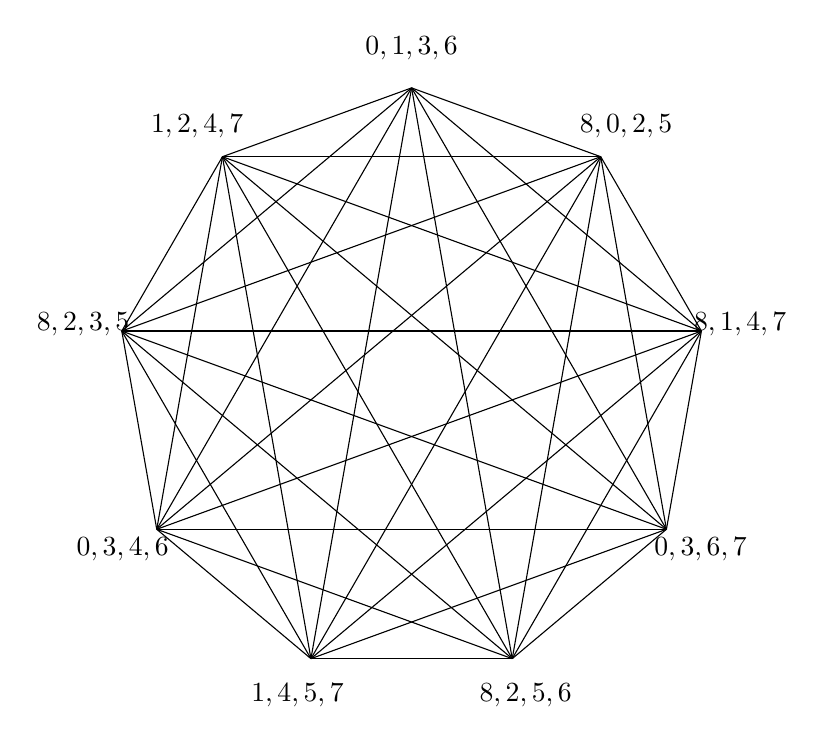
\begin{tikzpicture}
	\draw[black] ( 90  :  3.73719281884655 )--( 130  :  3.73719281884655 );
	\draw[black] ( 90  :  3.73719281884655 )--( 170  :  3.73719281884655 );
	\draw[black] ( 90  :  3.73719281884655 )--( 210  :  3.73719281884655 );
	\draw[black] ( 90  :  3.73719281884655 )--( 250  :  3.73719281884655 );
	\draw[black] ( 90  :  3.73719281884655 )--( 290  :  3.73719281884655 );
	\draw[black] ( 90  :  3.73719281884655 )--( 330  :  3.73719281884655 );
	\draw[black] ( 90  :  3.73719281884655 )--( 370  :  3.73719281884655 );
	\draw[black] ( 90  :  3.73719281884655 )--( 410  :  3.73719281884655 );
	\draw[black] ( 130  :  3.73719281884655 )--( 170  :  3.73719281884655 );
	\draw[black] ( 130  :  3.73719281884655 )--( 210  :  3.73719281884655 );
	\draw[black] ( 130  :  3.73719281884655 )--( 250  :  3.73719281884655 );
	\draw[black] ( 130  :  3.73719281884655 )--( 290  :  3.73719281884655 );
	\draw[black] ( 130  :  3.73719281884655 )--( 330  :  3.73719281884655 );
	\draw[black] ( 130  :  3.73719281884655 )--( 370  :  3.73719281884655 );
	\draw[black] ( 130  :  3.73719281884655 )--( 410  :  3.73719281884655 );
	\draw[black] ( 170  :  3.73719281884655 )--( 210  :  3.73719281884655 );
	\draw[black] ( 170  :  3.73719281884655 )--( 250  :  3.73719281884655 );
	\draw[black] ( 170  :  3.73719281884655 )--( 290  :  3.73719281884655 );
	\draw[black] ( 170  :  3.73719281884655 )--( 330  :  3.73719281884655 );
	\draw[black] ( 170  :  3.73719281884655 )--( 370  :  3.73719281884655 );
	\draw[black] ( 170  :  3.73719281884655 )--( 410  :  3.73719281884655 );
	\draw[black] ( 210  :  3.73719281884655 )--( 250  :  3.73719281884655 );
	\draw[black] ( 210  :  3.73719281884655 )--( 290  :  3.73719281884655 );
	\draw[black] ( 210  :  3.73719281884655 )--( 330  :  3.73719281884655 );
	\draw[black] ( 210  :  3.73719281884655 )--( 370  :  3.73719281884655 );
	\draw[black] ( 210  :  3.73719281884655 )--( 410  :  3.73719281884655 );
	\draw[black] ( 250  :  3.73719281884655 )--( 290  :  3.73719281884655 );
	\draw[black] ( 250  :  3.73719281884655 )--( 330  :  3.73719281884655 );
	\draw[black] ( 250  :  3.73719281884655 )--( 370  :  3.73719281884655 );
	\draw[black] ( 250  :  3.73719281884655 )--( 410  :  3.73719281884655 );
	\draw[black] ( 290  :  3.73719281884655 )--( 330  :  3.73719281884655 );
	\draw[black] ( 290  :  3.73719281884655 )--( 370  :  3.73719281884655 );
	\draw[black] ( 290  :  3.73719281884655 )--( 410  :  3.73719281884655 );
	\draw[black] ( 330  :  3.73719281884655 )--( 370  :  3.73719281884655 );
	\draw[black] ( 330  :  3.73719281884655 )--( 410  :  3.73719281884655 );
	\draw[black] ( 370  :  3.73719281884655 )--( 410  :  3.73719281884655 );
	\draw[fill=black] ( 90  :  4.23719281884655 ) node {$ {0, 1, 3, 6} $};
	\draw[fill=black] ( 130  :  4.23719281884655 ) node {$ {1, 2, 4, 7} $};
	\draw[fill=black] ( 170  :  4.23719281884655 ) node {$ {8, 2, 3, 5} $};
	\draw[fill=black] ( 210  :  4.23719281884655 ) node {$ {0, 3, 4, 6} $};
	\draw[fill=black] ( 250  :  4.23719281884655 ) node {$ {1, 4, 5, 7} $};
	\draw[fill=black] ( 290  :  4.23719281884655 ) node {$ {8, 2, 5, 6} $};
	\draw[fill=black] ( 330  :  4.23719281884655 ) node {$ {0, 3, 6, 7} $};
	\draw[fill=black] ( 370  :  4.23719281884655 ) node {$ {8, 1, 4, 7} $};
	\draw[fill=black] ( 410  :  4.23719281884655 ) node {$ {8, 0, 2, 5} $};
	
\end{tikzpicture}
	
	
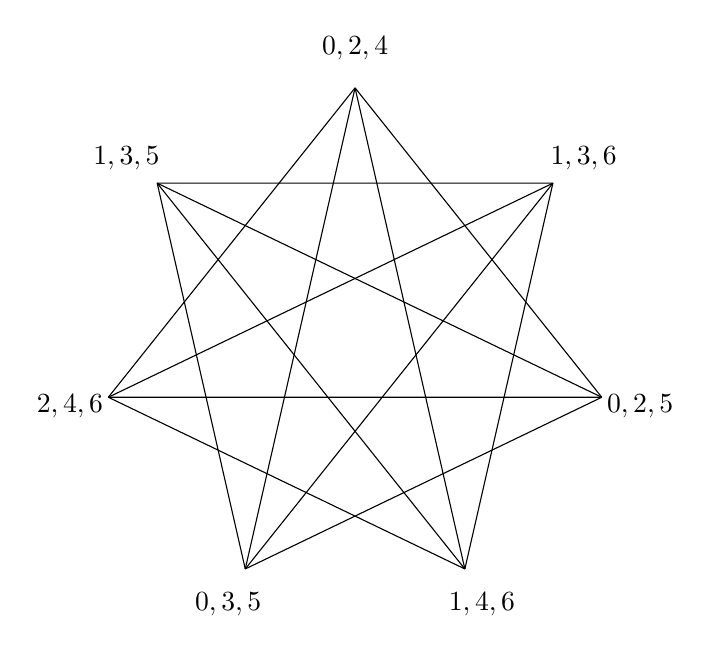
\begin{tikzpicture}
\draw[black] ( 90  :  3.21409584971604 )--( 1350/7  :  3.21409584971604 );
\draw[black] ( 90  :  3.21409584971604 )--( 1710/7  :  3.21409584971604 );
\draw[black] ( 90  :  3.21409584971604 )--( 2070/7  :  3.21409584971604 );
\draw[black] ( 90  :  3.21409584971604 )--( 2430/7  :  3.21409584971604 );
\draw[black] ( 990/7  :  3.21409584971604 )--( 1710/7  :  3.21409584971604 );
\draw[black] ( 990/7  :  3.21409584971604 )--( 2070/7  :  3.21409584971604 );
\draw[black] ( 990/7  :  3.21409584971604 )--( 2430/7  :  3.21409584971604 );
\draw[black] ( 990/7  :  3.21409584971604 )--( 2790/7  :  3.21409584971604 );
\draw[black] ( 1350/7  :  3.21409584971604 )--( 2070/7  :  3.21409584971604 );
\draw[black] ( 1350/7  :  3.21409584971604 )--( 2430/7  :  3.21409584971604 );
\draw[black] ( 1350/7  :  3.21409584971604 )--( 2790/7  :  3.21409584971604 );
\draw[black] ( 1710/7  :  3.21409584971604 )--( 2430/7  :  3.21409584971604 );
\draw[black] ( 1710/7  :  3.21409584971604 )--( 2790/7  :  3.21409584971604 );
\draw[black] ( 2070/7  :  3.21409584971604 )--( 2790/7  :  3.21409584971604 );
\draw[fill=black] ( 90  :  3.71409584971604 ) node {$ {0, 2, 4} $};
\draw[fill=black] ( 990/7  :  3.71409584971604 ) node {$ {1, 3, 5} $};
\draw[fill=black] ( 1350/7  :  3.71409584971604 ) node {$ {2, 4, 6} $};
\draw[fill=black] ( 1710/7  :  3.71409584971604 ) node {$ {0, 3, 5} $};
\draw[fill=black] ( 2070/7  :  3.71409584971604 ) node {$ {1, 4, 6} $};
\draw[fill=black] ( 2430/7  :  3.71409584971604 ) node {$ {0, 2, 5} $};
\draw[fill=black] ( 2790/7  :  3.71409584971604 ) node {$ {1, 3, 6} $};

\end{tikzpicture}
	
	
	
\begin{tikzpicture}
\draw[black] ( 90  :  2.62652780440377 )--( 234  :  2.62652780440377 );
\draw[black] ( 90  :  2.62652780440377 )--( 306  :  2.62652780440377 );
\draw[black] ( 162  :  2.62652780440377 )--( 306  :  2.62652780440377 );
\draw[black] ( 162  :  2.62652780440377 )--( 378  :  2.62652780440377 );
\draw[black] ( 234  :  2.62652780440377 )--( 378  :  2.62652780440377 );
\draw[fill=black] ( 90  :  3.12652780440377 ) node {$ {0, 2, 4} $};
\draw[fill=black] ( 162  :  3.12652780440377 ) node {$ {0, 1, 3} $};
\draw[fill=black] ( 234  :  3.12652780440377 ) node {$ {1, 2, 4} $};
\draw[fill=black] ( 306  :  3.12652780440377 ) node {$ {0, 2, 3} $};
\draw[fill=black] ( 378  :  3.12652780440377 ) node {$ {1, 3, 4} $};
\end{tikzpicture}
	
\begin{tikzpicture}
\draw[black] ( 90  :  2.62652780440377 )--( 162  :  2.62652780440377 );
\draw[black] ( 90  :  2.62652780440377 )--( 378  :  2.62652780440377 );
\draw[black] ( 162  :  2.62652780440377 )--( 234  :  2.62652780440377 );
\draw[black] ( 234  :  2.62652780440377 )--( 306  :  2.62652780440377 );
\draw[black] ( 306  :  2.62652780440377 )--( 378  :  2.62652780440377 );
\draw[fill=black] ( 90  :  3.12652780440377 ) node {$ {0, 1, 2} $};
\draw[fill=black] ( 162  :  3.12652780440377 ) node {$ {1, 2, 3} $};
\draw[fill=black] ( 234  :  3.12652780440377 ) node {$ {2, 3, 4} $};
\draw[fill=black] ( 306  :  3.12652780440377 ) node {$ {0, 3, 4} $};
\draw[fill=black] ( 378  :  3.12652780440377 ) node {$ {0, 1, 4} $};
\end{tikzpicture}	

\begin{tikzpicture}
\draw[black] ( 90  :  2.62652780440377 )--( 234  :  2.62652780440377 );
\draw[black] ( 90  :  2.62652780440377 )--( 306  :  2.62652780440377 );
\draw[black] ( 162  :  2.62652780440377 )--( 306  :  2.62652780440377 );
\draw[black] ( 162  :  2.62652780440377 )--( 378  :  2.62652780440377 );
\draw[black] ( 234  :  2.62652780440377 )--( 378  :  2.62652780440377 );
\draw[fill=black] ( 90  :  3.12652780440377 ) node {$ {0, 1, 2} $};
\draw[fill=black] ( 162  :  3.12652780440377 ) node {$ {1, 2, 3} $};
\draw[fill=black] ( 234  :  3.12652780440377 ) node {$ {2, 3, 4} $};
\draw[fill=black] ( 306  :  3.12652780440377 ) node {$ {0, 3, 4} $};
\draw[fill=black] ( 378  :  3.12652780440377 ) node {$ {0, 1, 4} $};
\end{tikzpicture}


	\begin{obs}
		Let $N$ be an integer necklace with $k$ beads of at most $n$ colours.  Then
		$$\bigcup_{i=1}^{k-1} JS(\mathcal{F}_N,i) \simeq K_k.$$
	\end{obs}
	
	\begin{conj}
		The degree of $JS(\mathcal{F}_n,i)$, denoted $d(JS(\mathcal{F}_n,i)))$, is
		$$|\{\sum_{\}$$
	\end{conj}
	
	\section{Initial Questions}
	
	
	
	\begin{question}
		Let $N_1$ and $N_2$ be distinct integer necklaces with $k$ beads of at most $n$ colours.  Let $G$ be the subgraph of $J(n,k,i)$ induced by $\mathcal{F}_{N_1} \cup \mathcal{F}_{N_2}$.  Does there exist an integer necklace $N'$ with $k'$ beads of at most $n'$ colours such that $G \simeq H$ where $H$ is the subgraph of $J(n',k',i')$ induced by $\mathcal{F}_{N'}$?
	\end{question}

	\begin{conjecture}[Probably Easy]
		If every difference in $\{1,\ldots,\floor{n/2}\}$ is in $N$, then $JS(\mathcal{F}_N,k-1) \simeq K_k$.
	\end{conjecture}
	
	\bibliographystyle{plain}
	\bibliography{bibliography}
	
\end{document}